\label{apx:a}

%\subsection{Graphiken, divers}
%
%\subsubsection{Aufstellung der Datengrundlage}
%
%\begin{figure*}[h]
%	\centering
%	\subfloat[kleiner Datensatz]{
%		\begin{minipage}[c][1.05\width]{
%			0.4\textwidth}
%			\centering
%	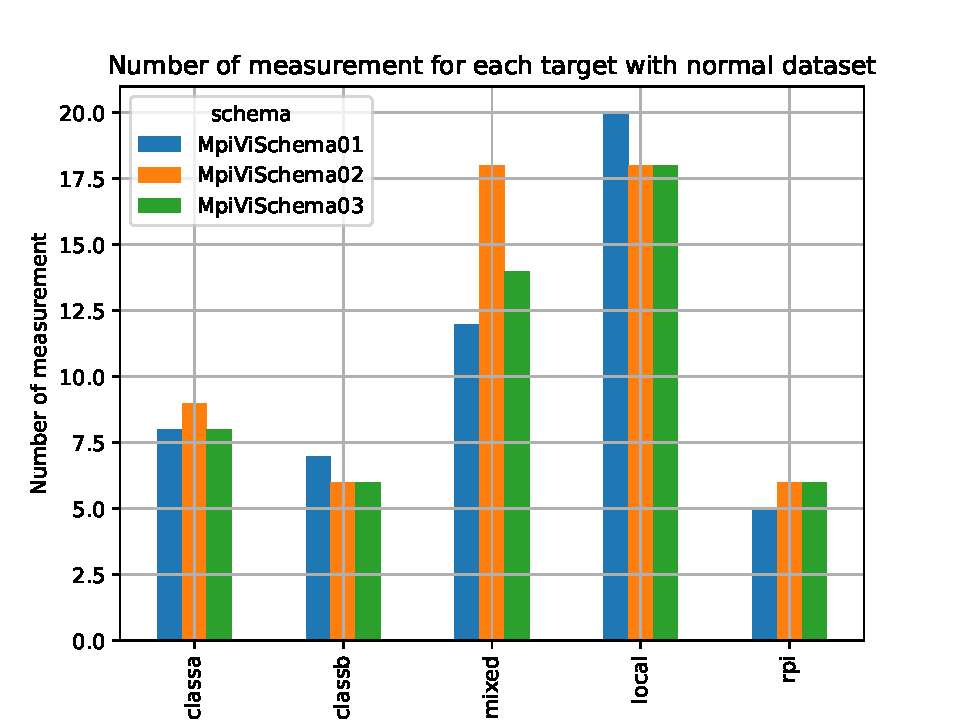
\includegraphics[width=1.1\textwidth]{./gen/img/ds/normal/number_measurement_target.pdf}
%		\end{minipage}}
%	\hfill
%	\subfloat[normaler Datensatz]{
%		\begin{minipage}[c][1.05\width]{
%			0.4\textwidth}
%			\centering
%	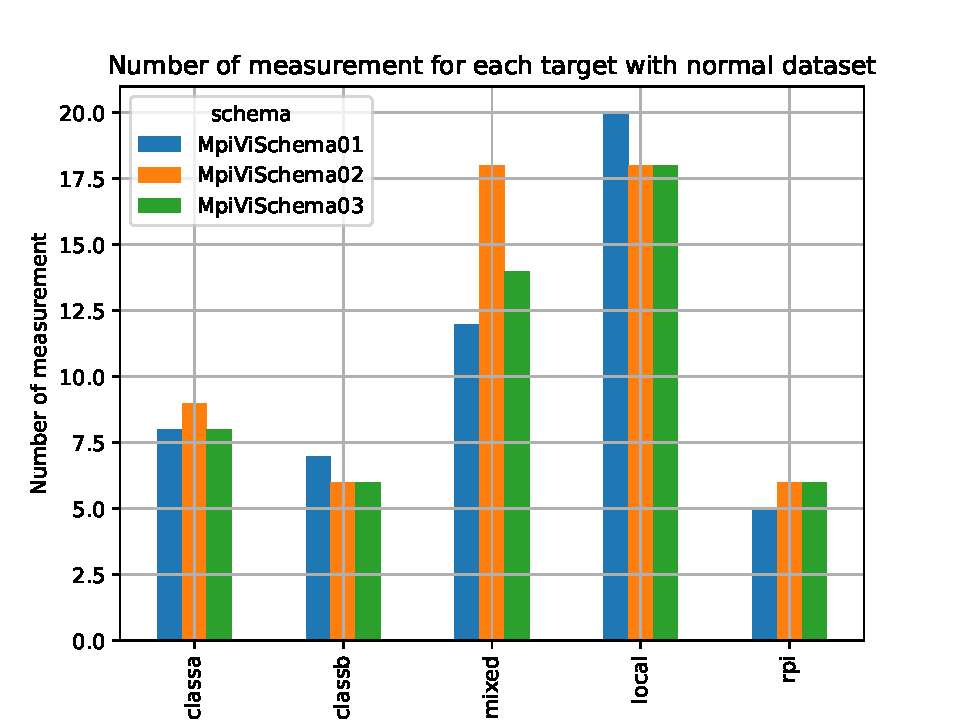
\includegraphics[width=1.1\textwidth]{./gen/img/ds/normal/number_measurement_target.pdf}
%		\end{minipage}}
%	\hfill
%	\centering
%	\subfloat[kleiner Datensatz]{
%		\begin{minipage}[c][1.05\width]{
%			0.4\textwidth}
%			\centering
%			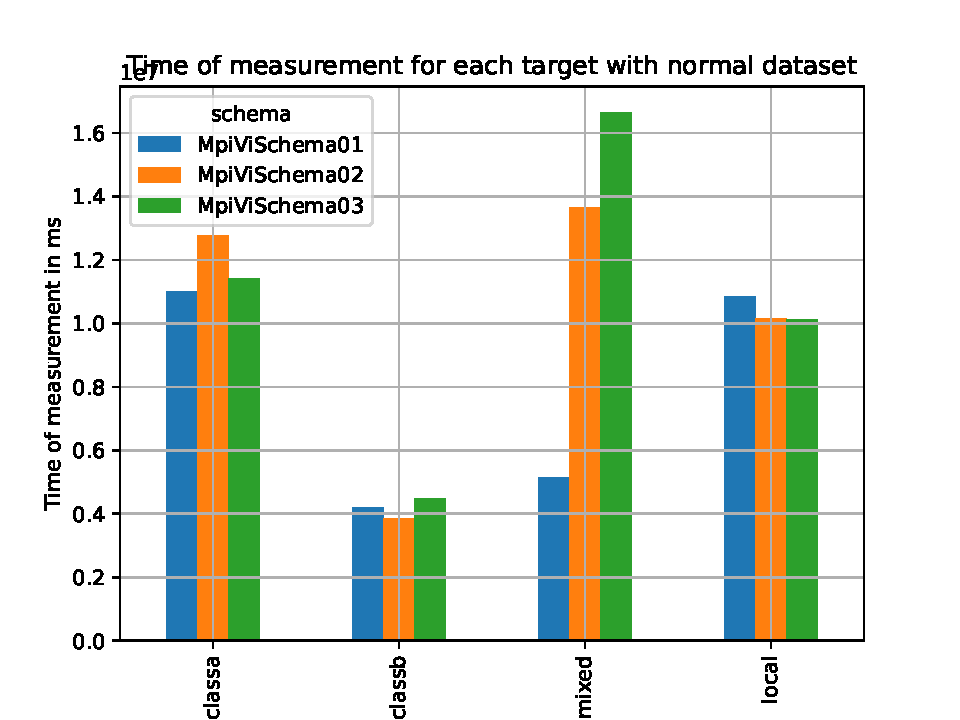
\includegraphics[width=1.1\textwidth]{./gen/img/ds/normal/runtime_measurement_target.pdf}
%		\end{minipage}}
%	\hfill
%	\subfloat[normaler Datensatz]{
%		\begin{minipage}[c][1.05\width]{
%			0.4\textwidth}
%			\centering
%			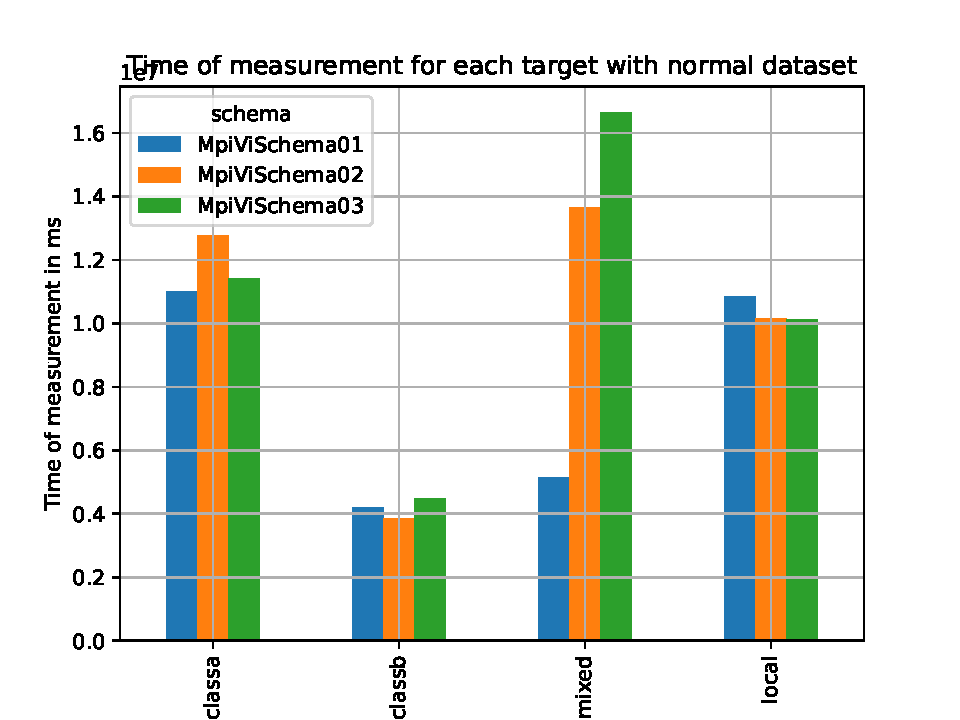
\includegraphics[width=1.1\textwidth]{./gen/img/ds/normal/runtime_measurement_target.pdf}
%		\end{minipage}}
%	\hfill
%	\caption{Anzahl\&Dauer an Messungen pro Rechenklasse}
%	\label{fig:3211} %TODO: add label
%\end{figure*}
%
%\subsubsection{Parametersweep: com\_interval}
%
%\begin{figure*}[h]
%	\centering
%	\subfloat[NUC, runtime\_vi/com\_interval, world\_size 2 \& 4]{
%		\begin{minipage}[c][1.05\width]{
%			0.4\textwidth}
%			\centering
%			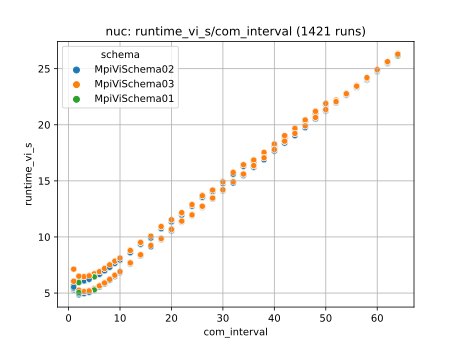
\includegraphics[width=1.1\textwidth]{./gen/img/nuc/small/scatterplot_com_interval_runtime_vi_s.pdf}
%		\end{minipage}}
%	\hfill
%	\subfloat[NUC, steps/com\_interval, world\_size 2 \& 4]{
%		\begin{minipage}[c][1.05\width]{
%			0.4\textwidth}
%			\centering
%			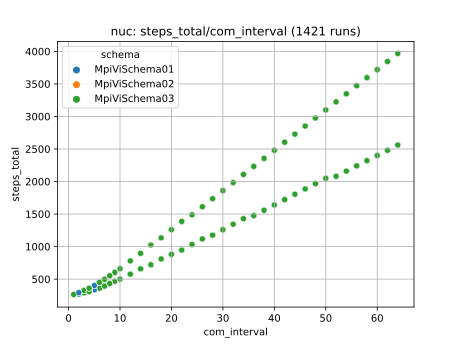
\includegraphics[width=1.1\textwidth]{./gen/img/nuc/small/scatterplot_com_interval_steps_total.pdf}
%		\end{minipage}}
%	\hfill
%	\caption{Parametersweep: co\_interval}
%	\label{fig:321} %TODO: add label
%\end{figure*}

\subsection{Gprahiken, Benchmark}
\label{sec:benchmark}

\subsubsection{Benchmak Datensatz small}

Die nachfolgenden Graphiken zeigen die Ergebnisse der Benchmarks für den Datensatz small.

\begin{figure*}
\centering
    \subfloat[HPC class A, runtime vs. world\_size]{
    	   \centering
    	   \includegraphics[width=0.33\textwidth]{./gen/img/hpcclassa/small/boxplot_world_size_runtime_vi_s.pdf}
    	   \label{fig:hpcAworldTimesmall}
    	\hspace{0pt}}
    \subfloat[HPC class B, runtime vs. world\_size]{
     	   \centering
     	   \includegraphics[width=0.33\textwidth]{./gen/img/hpcclassb/small/boxplot_world_size_runtime_vi_s.pdf}
     	  \label{fig:hpcBworldTimesmall}
     	\hspace{0pt}}
    \subfloat[HPC class mixed, runtime vs. world\_size]{
    	   \centering
    	   \includegraphics[width=0.33\textwidth]{./gen/img/hpcclassmixed/small/boxplot_world_size_runtime_vi_s.pdf}
    	   \label{fig:hpcMixedworldTimesmall}
    	}\\
    \subfloat[HPC class A runtime vs. com\_interval]{
    	\centering
    	   \includegraphics[width=0.33\textwidth]{./gen/img/hpcclassa/small/boxplot_com_interval_runtime_vi_s.pdf}
    	   \label{fig:hpcAcomTimesmall}
    	\hspace{0pt}}
    \subfloat[HPC class B runtime vs. com\_interval]{
    	\centering
     	   \includegraphics[width=0.33\textwidth]{./gen/img/hpcclassb/small/boxplot_com_interval_runtime_vi_s.pdf}
     	\hspace{0pt}}
    \subfloat[HPC class mixed runtime vs. com\_interval]{
    	\centering
    	   \includegraphics[width=0.33\textwidth]{./gen/img/hpcclassmixed/small/boxplot_com_interval_runtime_vi_s.pdf}
    	 \label{fig:hpcMixedcomTimesmall}
    	\hspace{0pt}}\\
    \subfloat[HPC class A max rss rank\_0 vs. world\_size]{
    	\centering
    	   \includegraphics[width=0.33\textwidth]{./gen/img/hpcclassa/small/boxplot_world_size_rss_max_rank0_mb.pdf}
    	   \label{fig:hpcAmaxRSSsmall}
    	\hspace{0pt}}
    \subfloat[HPC class B max rss rank\_0 vs. world\_size]{
    	\centering
     	   \includegraphics[width=0.33\textwidth]{./gen/img/hpcclassb/small/boxplot_world_size_rss_max_rank0_mb.pdf}
     	\hspace{0pt}}
    \subfloat[HPC class mixed max rss rank\_0 vs. world\_size]{
    	\centering
    	   \includegraphics[width=0.33\textwidth]{./gen/img/hpcclassmixed/small/boxplot_world_size_rss_max_rank0_mb.pdf}
    	\hspace{0pt}}\\
    \subfloat[HPC class A rss-sum vs. world\_size]{
    	\centering
    	   \includegraphics[width=0.33\textwidth]{./gen/img/hpcclassa/small/boxplot_world_size_rss_sum_all_mb.pdf}
    	   \label{fig:hpcAsumRSSsmall}
    	\hspace{0pt}}
    \subfloat[HPC class B rss-sum vs. world\_size]{
    	\centering
     	   \includegraphics[width=0.33\textwidth]{./gen/img/hpcclassb/small/boxplot_world_size_rss_sum_all_mb.pdf}
     	\hspace{0pt}}
    \subfloat[HPC class mixed rss-sum vs. world\_size]{
    	\centering
    	   \includegraphics[width=0.33\textwidth]{./gen/img/hpcclassmixed/small/boxplot_world_size_rss_sum_all_mb.pdf}
    	\hspace{0pt}}\\
    \caption{Comparison between HPC classes with dataset small}
\end{figure*}

\begin{figure*}
\centering
    \subfloat[NUC, runtime vs. world\_size]{
    	\centering
    	   \includegraphics[width=0.33\textwidth]{./gen/img/nuc/small/boxplot_world_size_runtime_vi_s.pdf}
    	   \label{fig:NUCworldTimesmall}
    	\hspace{0pt}}
    \subfloat[RPi, runtime vs. world\_size]{
    	\centering
     	   \includegraphics[width=0.33\textwidth]{./gen/img/rpi/small/boxplot_world_size_runtime_vi_s.pdf}
     	\hspace{0pt}}
    \subfloat[Local, runtime vs. world\_size]{
    	\centering
    	   \includegraphics[width=0.33\textwidth]{./gen/img/local/small/boxplot_world_size_runtime_vi_s.pdf}
    	}\\
    \subfloat[NUC runtime vs. com\_interval]{
    	\centering
    	   \includegraphics[width=0.33\textwidth]{./gen/img/nuc/small/boxplot_com_interval_runtime_vi_s.pdf}
    	   \label{fig:NUCcomTimesmall}
    	\hspace{0pt}}
    \subfloat[RPi runtime vs. com\_interval]{
    	\centering
     	   \includegraphics[width=0.33\textwidth]{./gen/img/rpi/small/boxplot_com_interval_runtime_vi_s.pdf}
     	\hspace{0pt}}
    \subfloat[Local runtime vs. com\_interval]{
    	\centering
    	   \includegraphics[width=0.33\textwidth]{./gen/img/local/small/boxplot_com_interval_runtime_vi_s.pdf}
    	\hspace{0pt}}\\
    \subfloat[NUC max rss rank\_0 vs. world\_size]{
    	 \centering
    	   \includegraphics[width=0.33\textwidth]{./gen/img/nuc/small/boxplot_world_size_rss_max_rank0_mb.pdf}
    	   \label{fig:NUCmaxRSSsmall}
    	\hspace{0pt}}
    \subfloat[RPi max rss rank\_0 vs. world\_size]{
    	 \centering
     	   \includegraphics[width=0.33\textwidth]{./gen/img/rpi/small/boxplot_world_size_rss_max_rank0_mb.pdf}
     	\hspace{0pt}}
    \subfloat[Local max rss rank\_0 vs. world\_size]{
    	\centering
    	   \includegraphics[width=0.33\textwidth]{./gen/img/local/small/boxplot_world_size_rss_max_rank0_mb.pdf}
    	\hspace{0pt}}\\
    \subfloat[NUC rss-sum vs. world\_size]{
    	 \centering
    	   \includegraphics[width=0.33\textwidth]{./gen/img/nuc/small/boxplot_world_size_rss_sum_all_mb.pdf}
    	   \label{fig:NUCsumRSSsmall}
    	\hspace{0pt}}
    \subfloat[RPi rss-sum vs. world\_size]{
    	\centering
     	   \includegraphics[width=0.33\textwidth]{./gen/img/rpi/small/boxplot_world_size_rss_sum_all_mb.pdf}
     	\hspace{0pt}}
    \subfloat[Local rss-sum vs. world\_size]{
    	\centering
    	   \includegraphics[width=0.33\textwidth]{./gen/img/local/small/boxplot_world_size_rss_sum_all_mb.pdf}
    	   \label{fig:LocalsumRSSsmall}
    	\hspace{0pt}}\\
    \caption{Comparison between NUC, RPi and Local with dataset small}
\end{figure*}

\begin{figure*}
\centering
    \subfloat[HPC class A, Iterations vs. world\_size]{
    	 \centering
    	   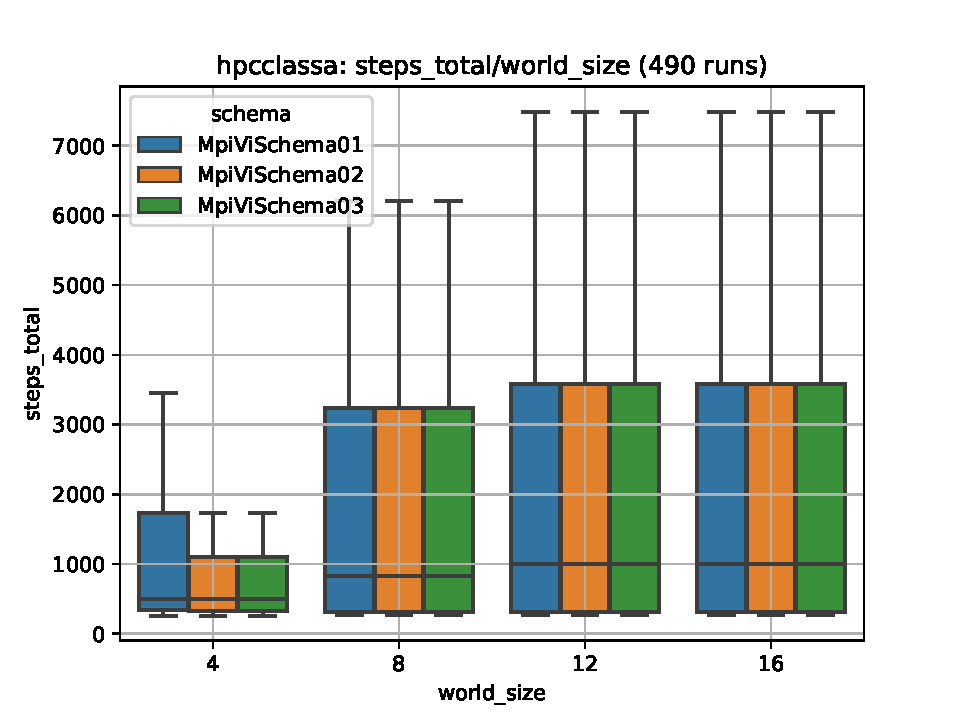
\includegraphics[width=0.33\textwidth]{./gen/img/hpcclassa/small/boxplot_world_size_steps_total.pdf}
    	   \label{fig:hpcAworldStepssmall}
    	\hspace{0pt}}
    \subfloat[HPC class B, Iterations vs. world\_size]{
     	   \centering
     	   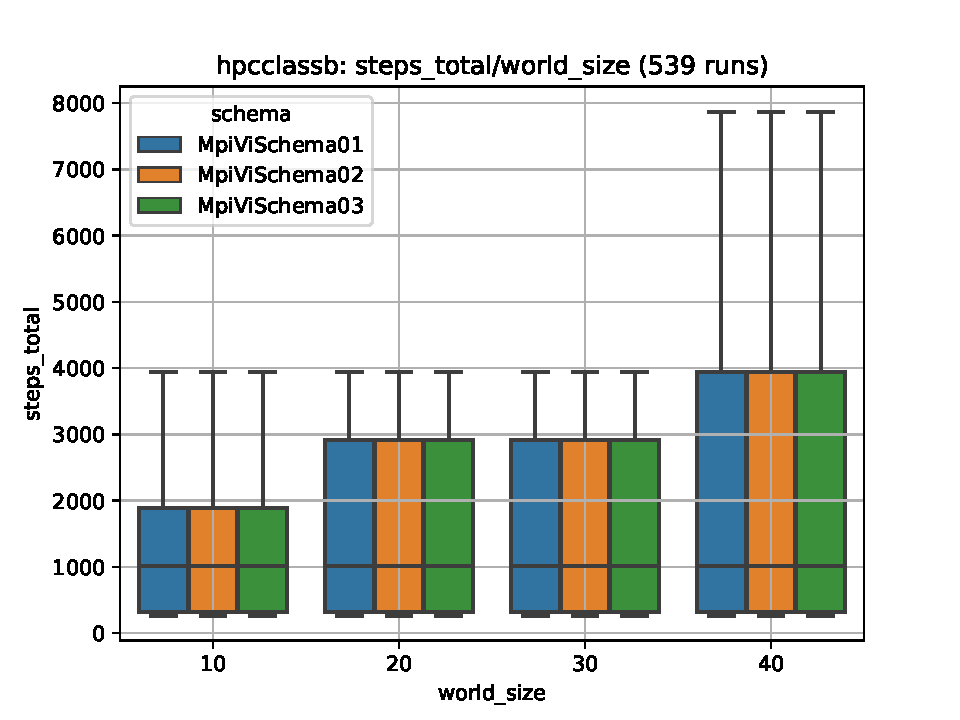
\includegraphics[width=0.33\textwidth]{./gen/img/hpcclassb/small/boxplot_world_size_steps_total.pdf}
     	\hspace{0pt}}
    \subfloat[HPC class mixed, Iterations vs. world\_size]{
    	   \centering
    	   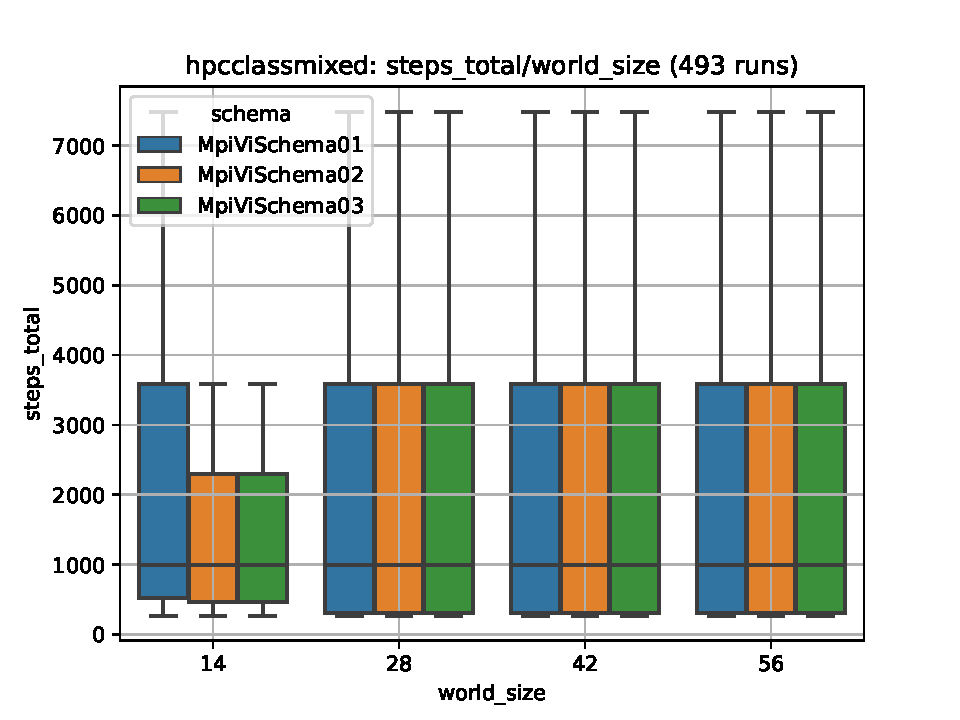
\includegraphics[width=0.33\textwidth]{./gen/img/hpcclassmixed/small/boxplot_world_size_steps_total.pdf}
    	\hspace{0pt}}\\
    \subfloat[HPC class A Iterations vs. com\_interval]{
    	   \centering
    	   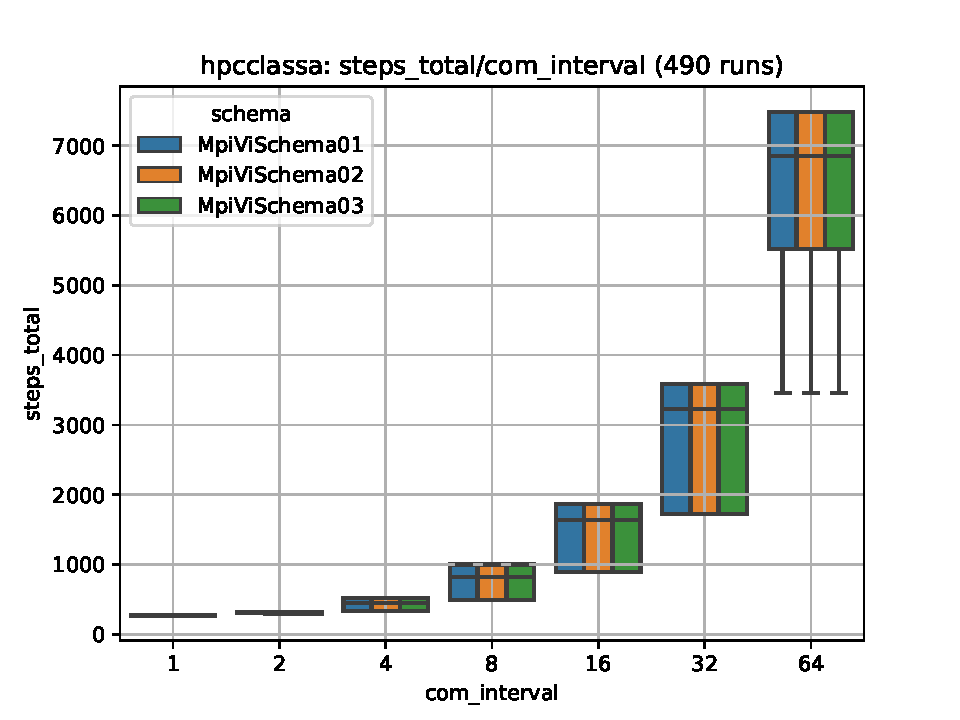
\includegraphics[width=0.33\textwidth]{./gen/img/hpcclassa/small/boxplot_com_interval_steps_total.pdf}
    	   \label{fig:hpcAcomStepssmall}
    	\hspace{0pt}}
    \subfloat[HPC class B Iterations vs. com\_interval]{
     	   \centering
     	   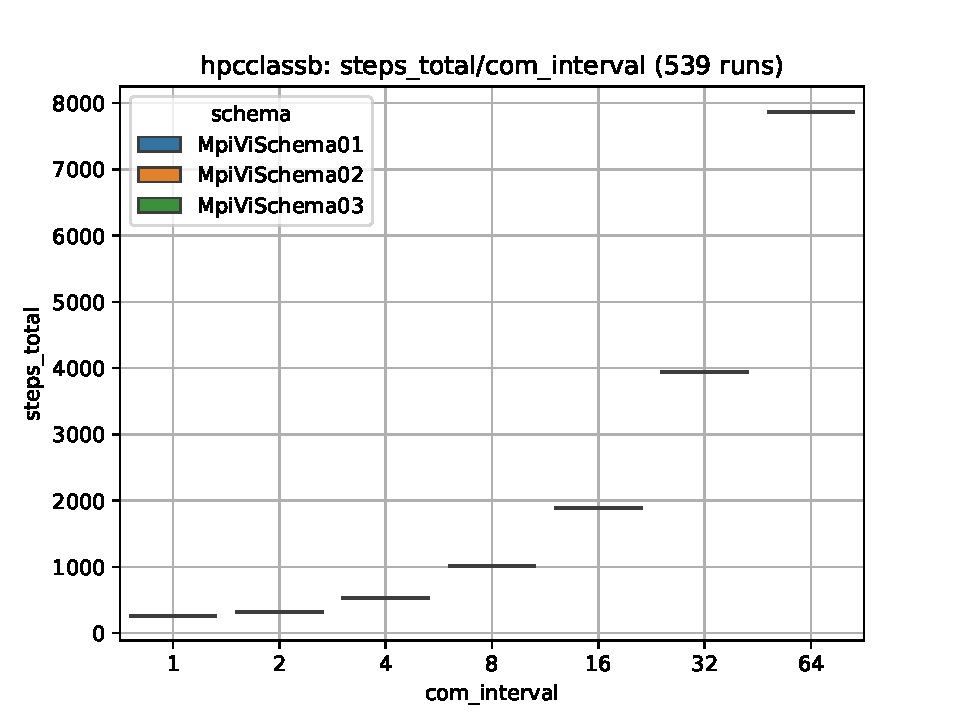
\includegraphics[width=0.33\textwidth]{./gen/img/hpcclassb/small/boxplot_com_interval_steps_total.pdf}
     	\hspace{0pt}}
    \subfloat[HPC class mixed Iterations vs. com\_interval]{
    	   \centering
    	   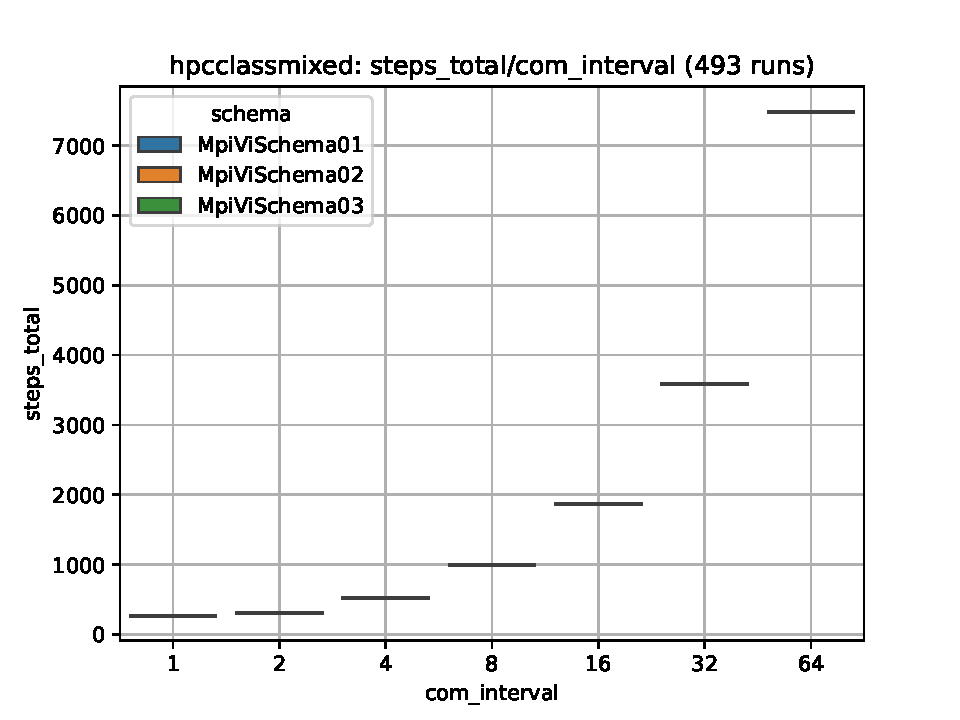
\includegraphics[width=0.33\textwidth]{./gen/img/hpcclassmixed/small/boxplot_com_interval_steps_total.pdf}
    	\hspace{0pt}}\\
    \subfloat[HPC class A J-diff maxnorm vs. world\_size]{
    	   \centering
    	   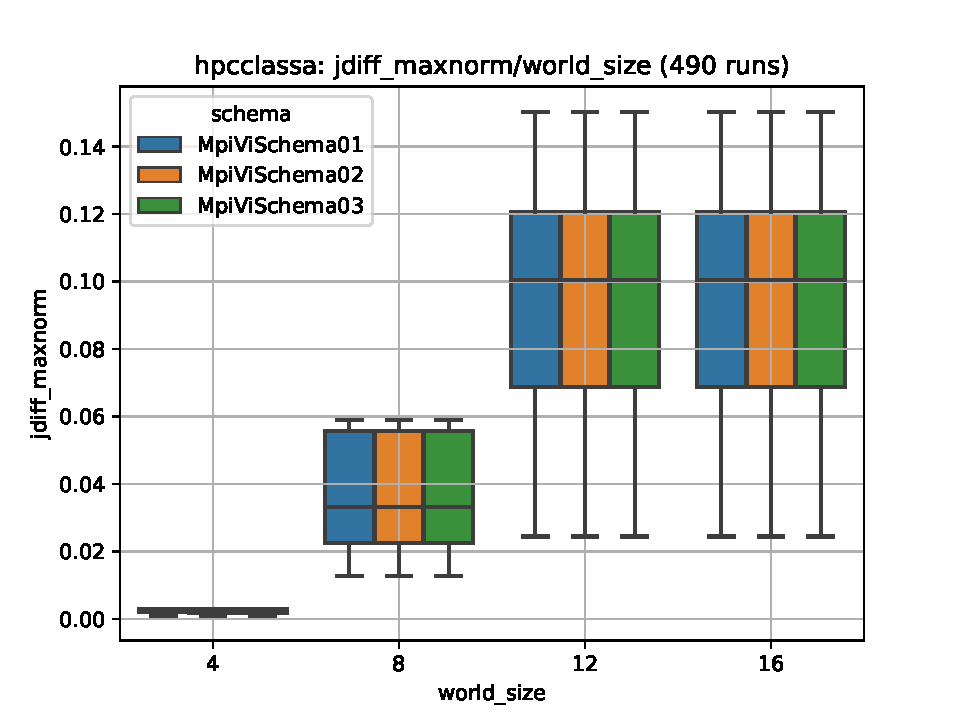
\includegraphics[width=0.33\textwidth]{./gen/img/hpcclassa/small/boxplot_world_size_jdiff_maxnorm.pdf}
    	\hspace{0pt}}
    \subfloat[HPC class B J-diff maxnorm vs. world\_size]{
     	   \centering
     	   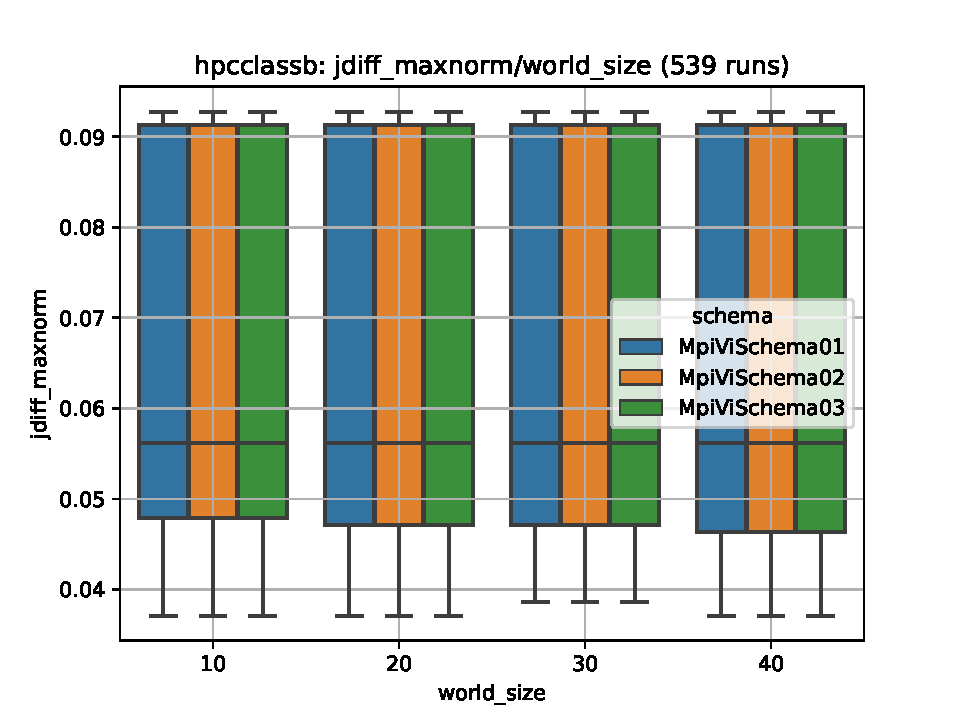
\includegraphics[width=0.33\textwidth]{./gen/img/hpcclassb/small/boxplot_world_size_jdiff_maxnorm.pdf}
     	\hspace{0pt}}
    \subfloat[HPC class mixed J-diff maxnorm vs. world\_size]{
    	   \centering
    	   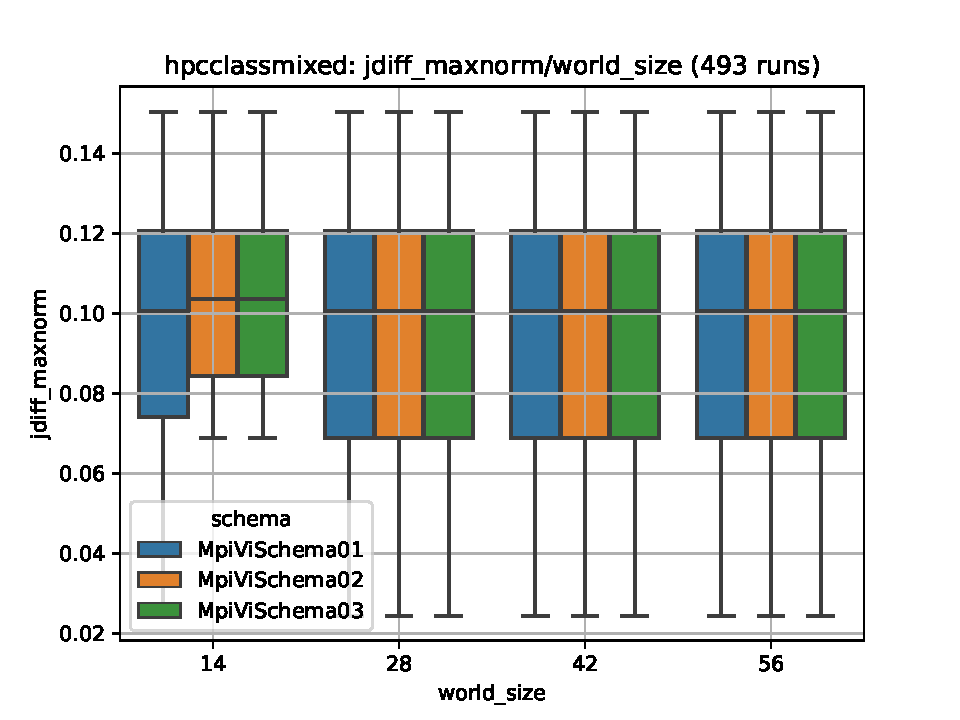
\includegraphics[width=0.33\textwidth]{./gen/img/hpcclassmixed/small/boxplot_world_size_jdiff_maxnorm.pdf}
    	\hspace{0pt}}\\
    \subfloat[HPC class A J-diff maxnorm vs. com\_interval]{
    	   \centering
    	   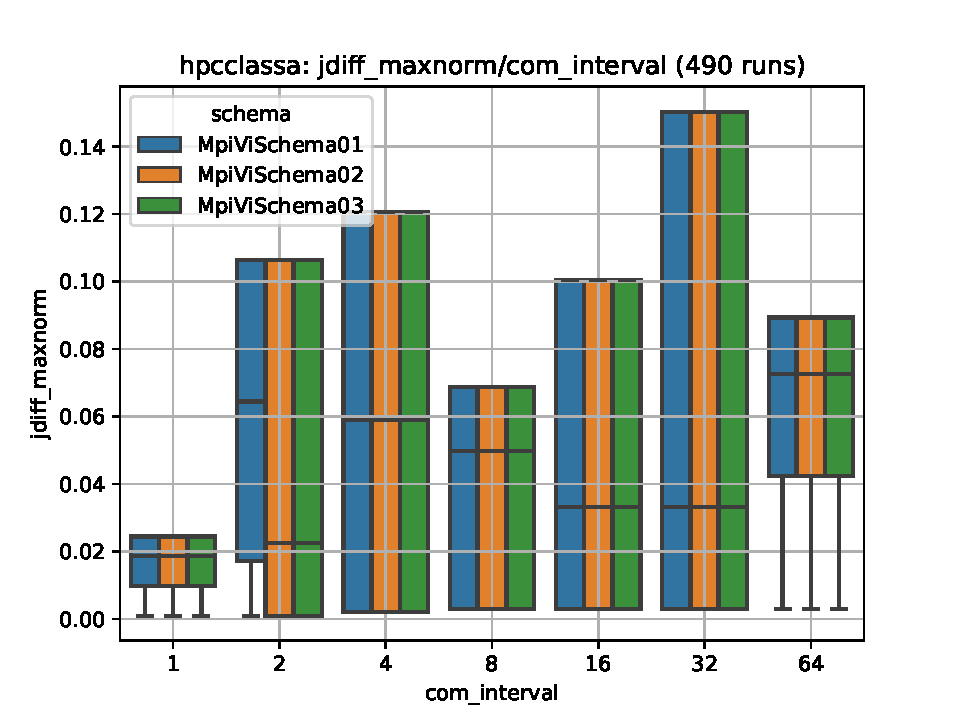
\includegraphics[width=0.33\textwidth]{./gen/img/hpcclassa/small/boxplot_com_interval_jdiff_maxnorm.pdf}
    	   \label{fig:hpcAcomJdiffssmall}
    	\hspace{0pt}}
    \subfloat[HPC class B J-diff maxnorm vs. com\_interval]{
     	   \centering
     	   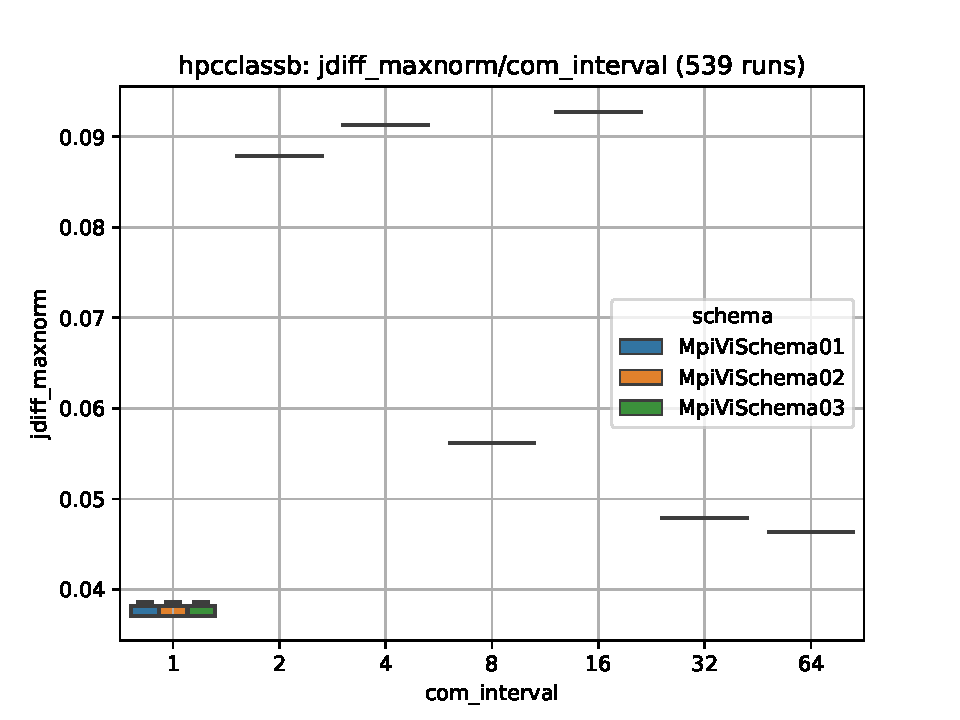
\includegraphics[width=0.33\textwidth]{./gen/img/hpcclassb/small/boxplot_com_interval_jdiff_maxnorm.pdf}
     	\hspace{0pt}}
    \subfloat[HPC class mixed J-diff maxnorm vs. com\_interval]{
    	   \centering
    	   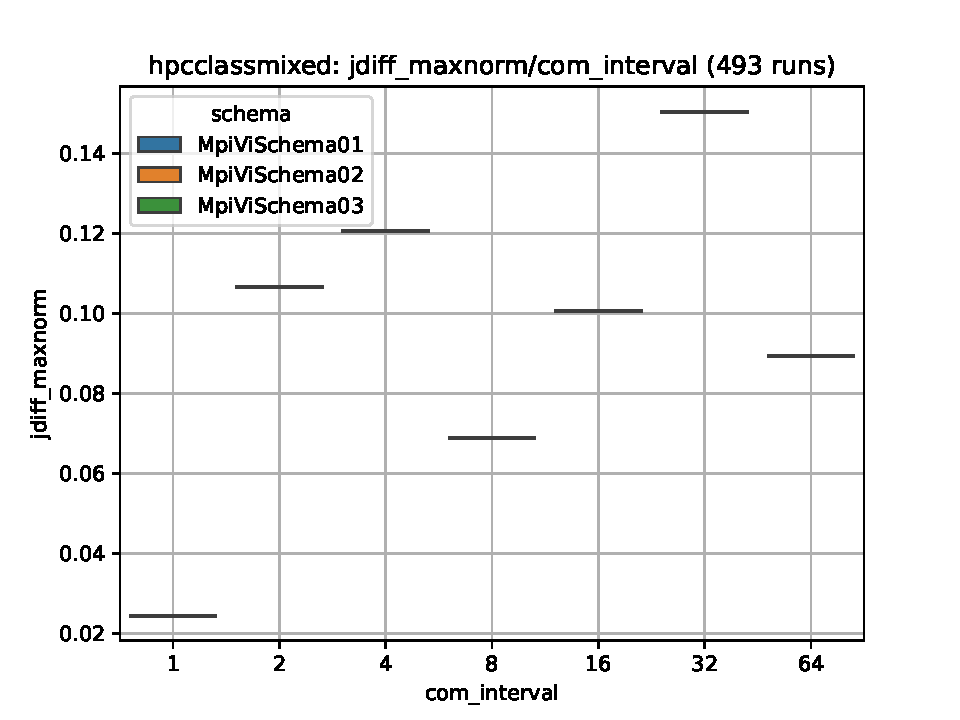
\includegraphics[width=0.33\textwidth]{./gen/img/hpcclassmixed/small/boxplot_com_interval_jdiff_maxnorm.pdf}
    	\hspace{0pt}}\\
    \caption{Comparison between HPC classes with dataset small}
\end{figure*}

\begin{figure*}
\centering
    \subfloat[NUC, Iterations vs. world\_size]{
    	   \centering
    	   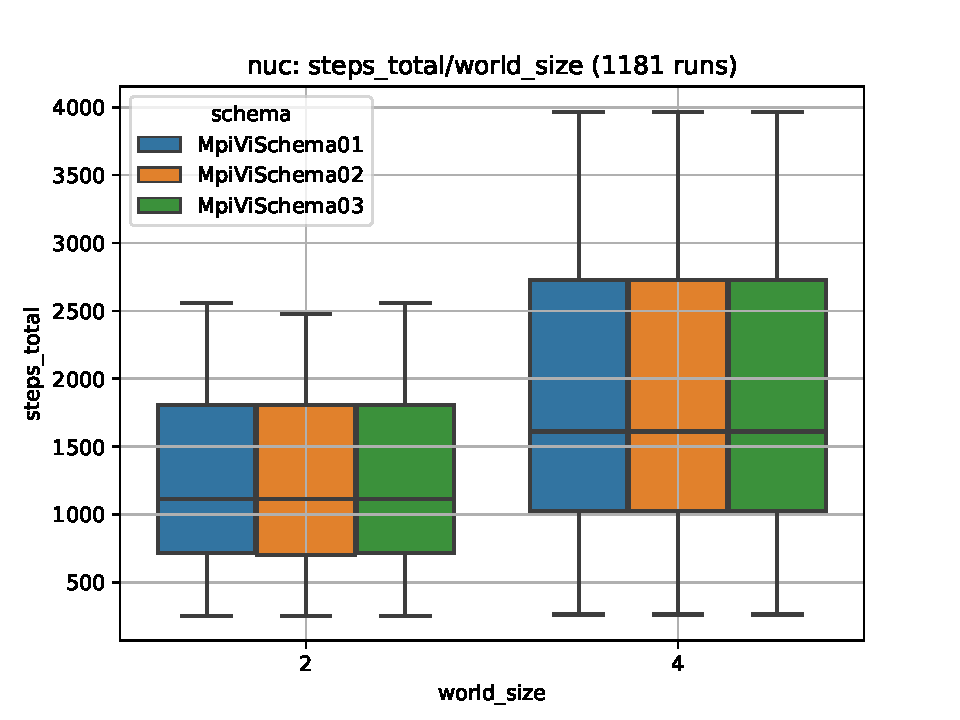
\includegraphics[width=0.33\textwidth]{./gen/img/nuc/small/boxplot_world_size_steps_total.pdf}
    	  \label{fig:NUCStepWorldSizesmall}
    	\hspace{0pt}}
    \subfloat[RPi, Iterations vs. world\_size]{
     	   \centering
     	   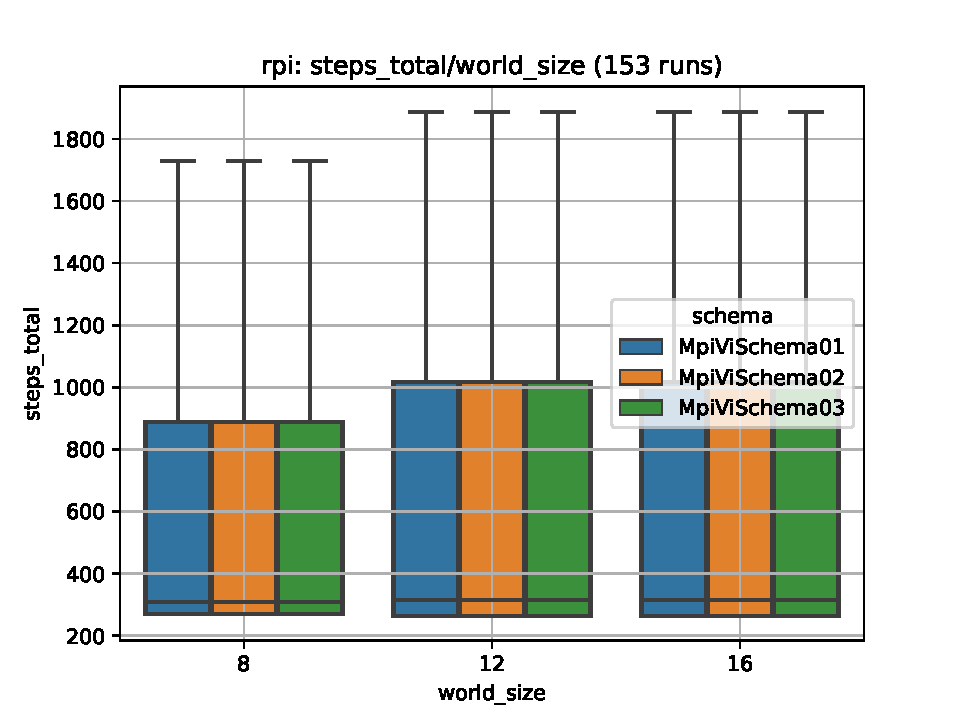
\includegraphics[width=0.33\textwidth]{./gen/img/rpi/small/boxplot_world_size_steps_total.pdf}
     	\hspace{0pt}}
    \subfloat[Local, Iterations vs. world\_size]{
    	   \centering
    	   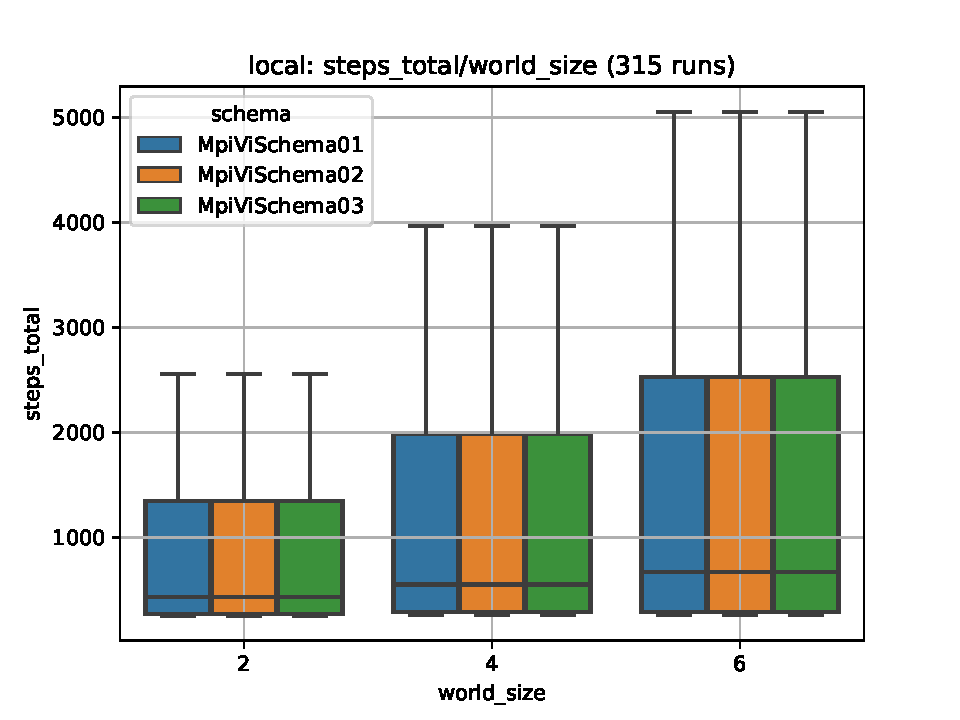
\includegraphics[width=0.33\textwidth]{./gen/img/local/small/boxplot_world_size_steps_total.pdf}
    	\hspace{0pt}}\\
    \subfloat[NUC Iterations vs. com\_interval]{
    	   \centering
    	   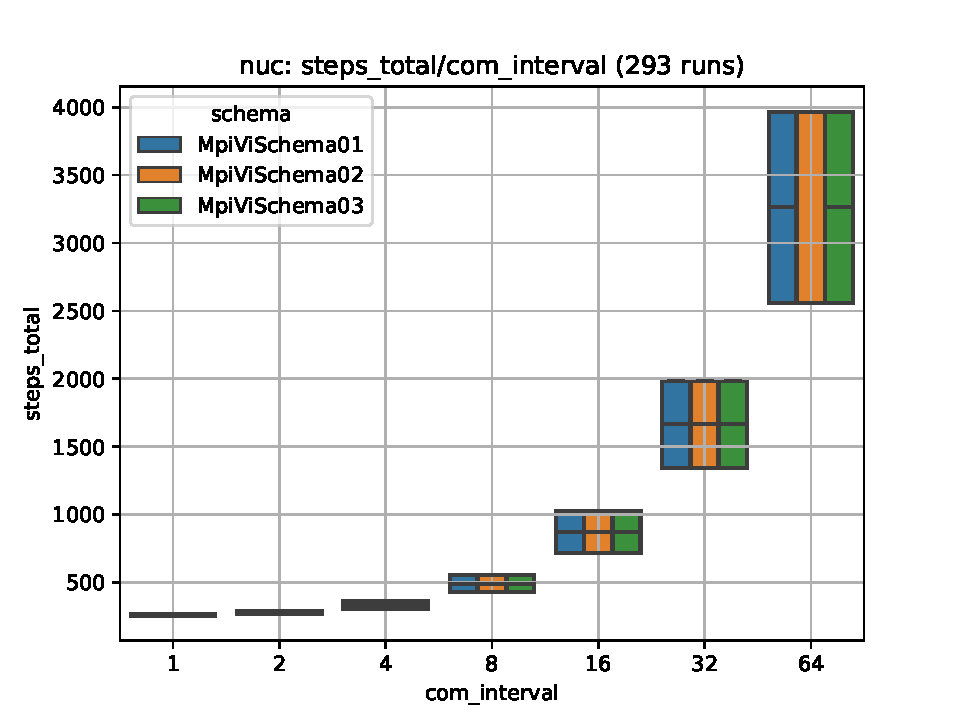
\includegraphics[width=0.33\textwidth]{./gen/img/nuc/small/boxplot_com_interval_steps_total.pdf}
    	   \label{fig:NUCIterationWorldSizesmall}
    	\hspace{0pt}}
    \subfloat[RPi Iterations vs. com\_interval]{
     	   \centering
     	   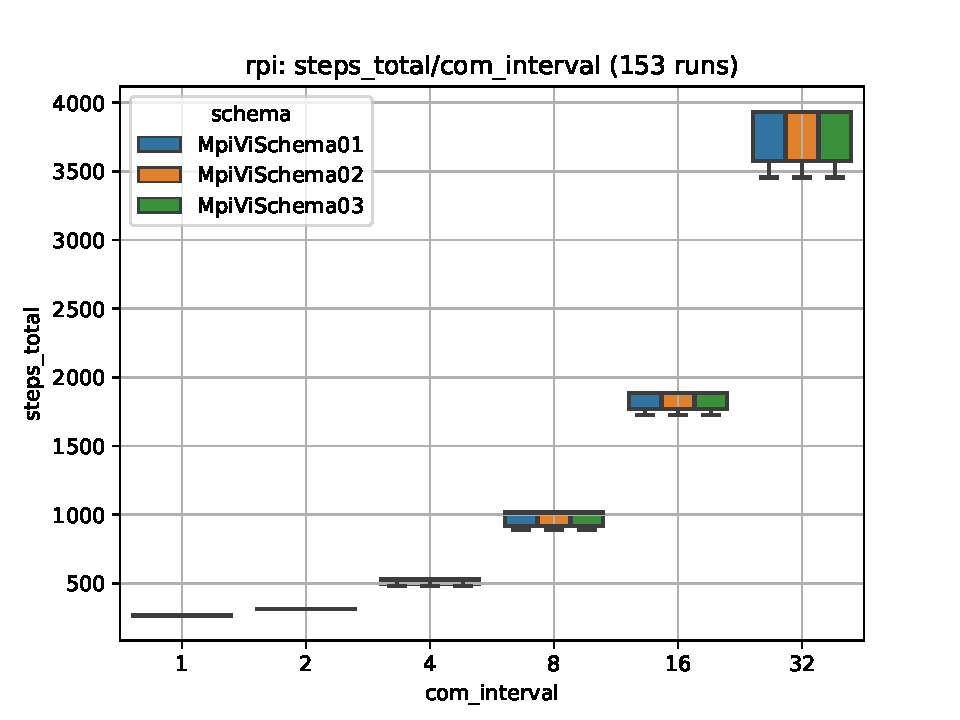
\includegraphics[width=0.33\textwidth]{./gen/img/rpi/small/boxplot_com_interval_steps_total.pdf}
     	\hspace{0pt}}
    \subfloat[Local Iterations vs. com\_interval]{
    	   \centering
    	   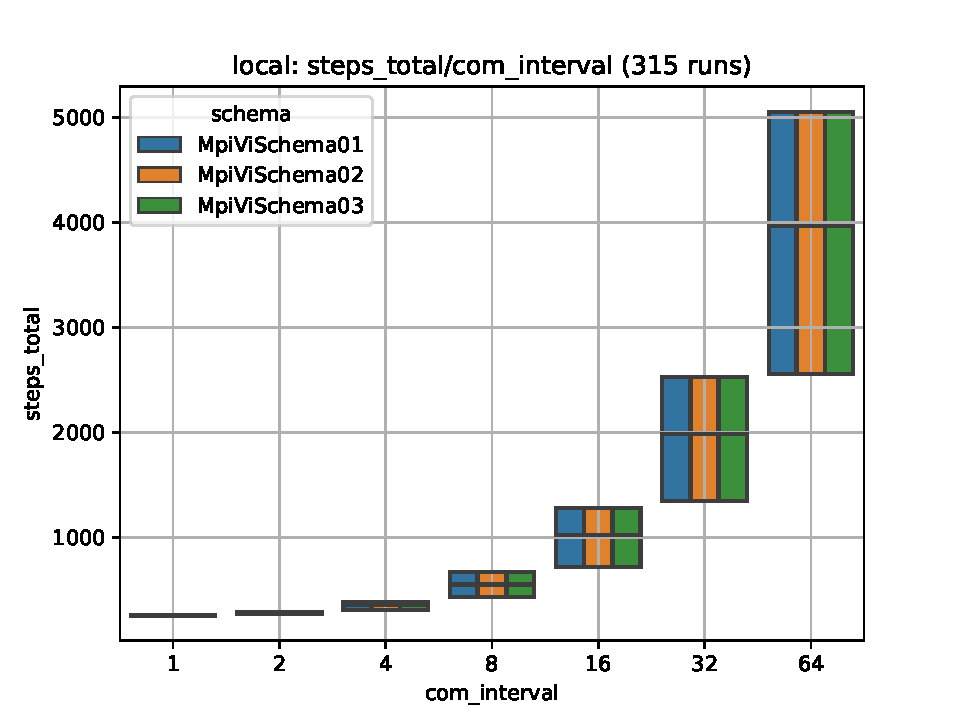
\includegraphics[width=0.33\textwidth]{./gen/img/local/small/boxplot_com_interval_steps_total.pdf}
    	}\\
    \subfloat[NUC J-diff maxnorm vs. world\_size]{
    	   \centering
    	   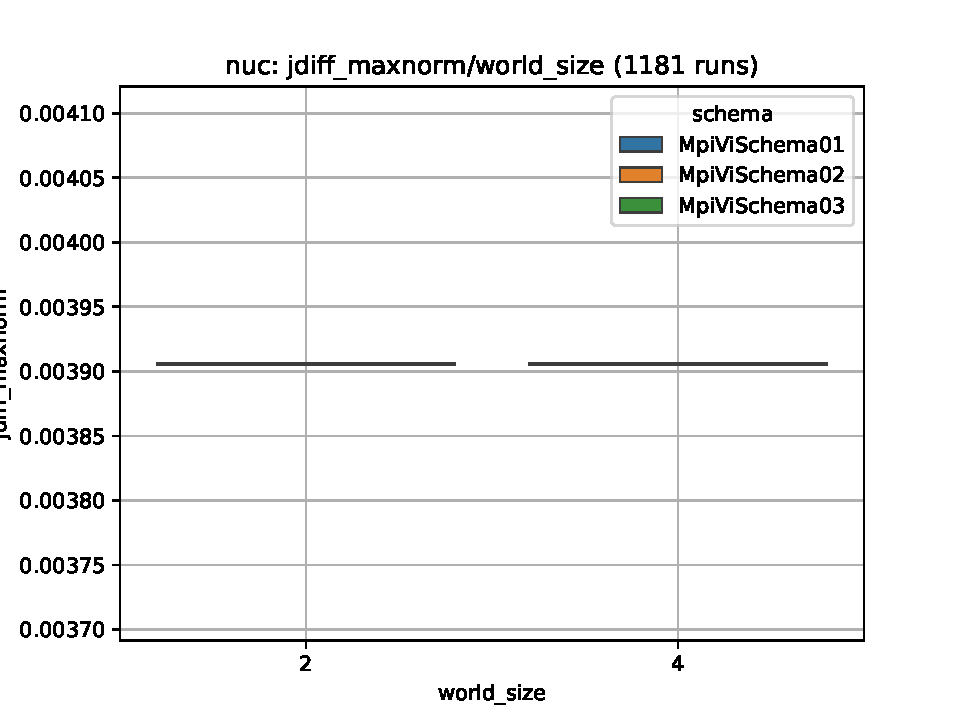
\includegraphics[width=0.33\textwidth]{./gen/img/nuc/small/boxplot_world_size_jdiff_maxnorm.pdf}
    	\hspace{0pt}}
    \subfloat[RPi J-diff maxnorm vs. world\_size]{
     	   \centering
     	   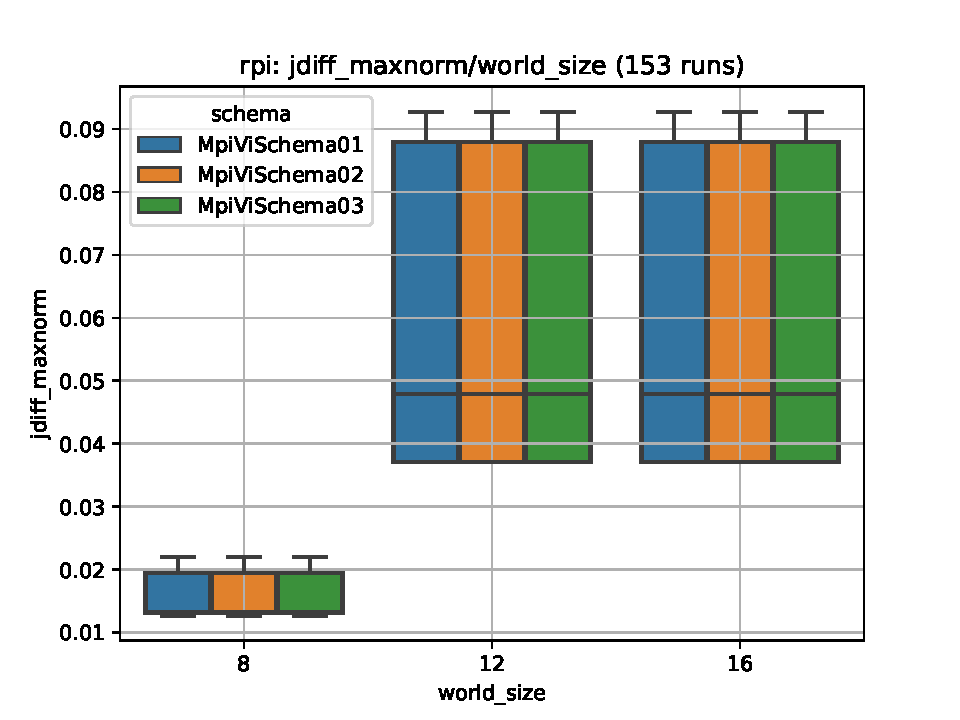
\includegraphics[width=0.33\textwidth]{./gen/img/rpi/small/boxplot_world_size_jdiff_maxnorm.pdf}
     	\hspace{0pt}}
    \subfloat[Local J-diff maxnorm vs. world\_size]{
    	   \centering
    	   \includegraphics[width=0.33\textwidth]{./gen/img/local/small/boxplot_world_size_jdiff_maxnorm.pdf}
    	\hspace{0pt}}\\
    \subfloat[NUC J-diff maxnorm vs. com\_interval]{
    	   \centering
    	   \includegraphics[width=0.33\textwidth]{./gen/img/nuc/small/boxplot_com_interval_jdiff_maxnorm.pdf}
    	\hspace{0pt}}
        \label{fig:hNUCcomJdiffssmall}
    \subfloat[RPi J-diff maxnorm vs. com\_interval]{
     	   \centering
     	   \includegraphics[width=0.33\textwidth]{./gen/img/rpi/small/boxplot_com_interval_jdiff_maxnorm.pdf}
     	    \hspace{0pt}}
    \subfloat[Local J-diff maxnorm vs. com\_interval]{
    	   \centering
    	   \includegraphics[width=0.33\textwidth]{./gen/img/local/small/boxplot_com_interval_jdiff_maxnorm.pdf}
    	    \hspace{0pt}}\\
    \caption{Comparison between NUC, RPi and Local with dataset small}
\end{figure*}

\subsubsection{Benchmark Datensatz normal}

Die nachfolgenden Graphiken zeigen die Ergebnisse der Benchmarks für den Datensatz normal.

\begin{figure*}
\centering
    \subfloat[HPC class A, runtime vs. world\_size]{
    	   \centering
    	   \includegraphics[width=0.33\textwidth]{./gen/img/hpcclassa/normal/boxplot_world_size_runtime_vi_s.pdf}
    	   \label{fig:hpcAworldTimenormal}
    	\hspace{0pt}}
    \subfloat[HPC class B, runtime vs. world\_size]{
     	   \centering
     	   \includegraphics[width=0.33\textwidth]{./gen/img/hpcclassb/normal/boxplot_world_size_runtime_vi_s.pdf}
     	\hspace{0pt}}
    \subfloat[HPC class mixed, runtime vs. world\_size]{
    	   \centering
    	   \includegraphics[width=0.33\textwidth]{./gen/img/hpcclassmixed/normal/boxplot_world_size_runtime_vi_s.pdf}
    	\hspace{0pt}}\\
    \subfloat[HPC class A runtime vs. com\_interval]{
    	   \centering
    	   \includegraphics[width=0.33\textwidth]{./gen/img/hpcclassa/normal/boxplot_com_interval_runtime_vi_s.pdf}
    	   \label{fig:hpcAcomTimenormal}
    	\hspace{0pt}}
    \subfloat[HPC class B runtime vs. com\_interval]{
     	   \centering
     	   \includegraphics[width=0.33\textwidth]{./gen/img/hpcclassb/normal/boxplot_com_interval_runtime_vi_s.pdf}
     	\hspace{0pt}}
    \subfloat[HPC class mixed runtime vs. com\_interval]{
    	   \centering
    	   \includegraphics[width=0.33\textwidth]{./gen/img/hpcclassmixed/normal/boxplot_com_interval_runtime_vi_s.pdf}
    	\hspace{0pt}}\\
    \subfloat[HPC class A max rss rank\_0 vs. world\_size]{
    	   \centering
    	   \includegraphics[width=0.33\textwidth]{./gen/img/hpcclassa/normal/boxplot_world_size_rss_max_rank0_mb.pdf}
    	   \label{fig:hpcAmaxRSSnormal}
    	\hspace{0pt}}
    \subfloat[HPC class B max rss rank\_0 vs. world\_size]{
     	   \centering
     	   \includegraphics[width=0.33\textwidth]{./gen/img/hpcclassb/normal/boxplot_world_size_rss_max_rank0_mb.pdf}
     	\hspace{0pt}}
    \subfloat[HPC class mixed max rss rank\_0 vs. world\_size]{
    	   \centering
    	   \includegraphics[width=0.33\textwidth]{./gen/img/hpcclassmixed/normal/boxplot_world_size_rss_max_rank0_mb.pdf}
    	\hspace{0pt}}\\
    \subfloat[HPC class A rss-sum vs. world\_size]{
    	   \centering
    	   \includegraphics[width=0.33\textwidth]{./gen/img/hpcclassa/normal/boxplot_world_size_rss_sum_all_mb.pdf}
    	   \label{fig:hpcAsumRSSnormal}
    	\hspace{0pt}}
    \subfloat[HPC class B rss-sum vs. world\_size]{
     	   \centering
     	   \includegraphics[width=0.33\textwidth]{./gen/img/hpcclassb/normal/boxplot_world_size_rss_sum_all_mb.pdf}
     	\hspace{0pt}}
    \subfloat[HPC class mixed rss-sum vs. world\_size]{
    	   \centering
    	   \includegraphics[width=0.33\textwidth]{./gen/img/hpcclassmixed/normal/boxplot_world_size_rss_sum_all_mb.pdf}
    	\hspace{0pt}}\\
    \caption{Comparison between HPC classes with dataset normal}
\end{figure*}

\begin{figure*}
\centering
    \subfloat[NUC, runtime vs. world\_size]{
    	   \centering
    	   \includegraphics[width=0.33\textwidth]{./gen/img/nuc/normal/boxplot_world_size_runtime_vi_s.pdf}
    	   \label{fig:NUCworldTimenormal}
    	\hspace{0pt}}
    \subfloat[RPi, runtime vs. world\_size]{
     	   \centering
     	   \includegraphics[width=0.33\textwidth]{./gen/img/rpi/normal/boxplot_world_size_runtime_vi_s.pdf}
     	\hspace{0pt}}
    \subfloat[Local, runtime vs. world\_size]{
    	   \centering
    	   \includegraphics[width=0.33\textwidth]{./gen/img/local/normal/boxplot_world_size_runtime_vi_s.pdf}
    	\hspace{0pt}}\\
    \subfloat[NUC runtime vs. com\_interval]{
    	   \centering
    	   \includegraphics[width=0.33\textwidth]{./gen/img/nuc/normal/boxplot_com_interval_runtime_vi_s.pdf}
    	   \label{fig:NUCcomTimenormal}
    	\hspace{0pt}}
    \subfloat[RPi runtime vs. com\_interval]{
     	   \centering
     	   \includegraphics[width=0.33\textwidth]{./gen/img/rpi/normal/boxplot_com_interval_runtime_vi_s.pdf}
     	\hspace{0pt}}
    \subfloat[Local runtime vs. com\_interval]{
    	   \centering
    	   \includegraphics[width=0.33\textwidth]{./gen/img/local/normal/boxplot_com_interval_runtime_vi_s.pdf}
    	\hspace{0pt}}\\
    \subfloat[NUC max rss rank\_0 vs. world\_size]{
    	   \centering
    	   \includegraphics[width=0.33\textwidth]{./gen/img/nuc/normal/boxplot_world_size_rss_max_rank0_mb.pdf}
    	   \label{fig:NUCmaxRSSnormal}
    	\hspace{0pt}}
    \subfloat[RPi max rss rank\_0 vs. world\_size]{
     	   \centering
     	   \includegraphics[width=0.33\textwidth]{./gen/img/rpi/normal/boxplot_world_size_rss_max_rank0_mb.pdf}
     	\hspace{0pt}}
    \subfloat[Local max rss rank\_0 vs. world\_size]{
    	   \centering
    	   \includegraphics[width=0.33\textwidth]{./gen/img/local/normal/boxplot_world_size_rss_max_rank0_mb.pdf}
    	\hspace{0pt}}\\
    \subfloat[NUC rss-sum vs. world\_size]{
    	   \centering
    	   \includegraphics[width=0.33\textwidth]{./gen/img/nuc/normal/boxplot_world_size_rss_sum_all_mb.pdf}
    	   \label{fig:NUCsumRSSnormal}
    	\hspace{0pt}}
    \subfloat[RPi rss-sum vs. world\_size]{
     	   \centering
     	   \includegraphics[width=0.33\textwidth]{./gen/img/rpi/normal/boxplot_world_size_rss_sum_all_mb.pdf}
     	\hspace{0pt}}
    \subfloat[Local rss-sum vs. world\_size]{
    	   \centering
    	   \includegraphics[width=0.33\textwidth]{./gen/img/local/normal/boxplot_world_size_rss_sum_all_mb.pdf}
    	\hspace{0pt}}\\
    \caption{Comparison between NUC, RPi and Local with dataset normal}
\end{figure*}

\begin{figure*}
\centering
    \subfloat[HPC class A, Iterations vs. world\_size]{
    	   \centering
    	   \includegraphics[width=0.33\textwidth]{./gen/img/hpcclassa/normal/boxplot_world_size_steps_total.pdf}
    	\hspace{0pt}}
    \subfloat[HPC class B, Iterations vs. world\_size]{
     	   \centering
     	   \includegraphics[width=0.33\textwidth]{./gen/img/hpcclassb/normal/boxplot_world_size_steps_total.pdf}
     	\hspace{0pt}}
    \subfloat[HPC class mixed, Iterations vs. world\_size]{
    	   \centering
    	   \includegraphics[width=0.33\textwidth]{./gen/img/hpcclassmixed/normal/boxplot_world_size_steps_total.pdf}
    	\hspace{0pt}}\\
    \subfloat[HPC class A Iterations vs. com\_interval]{
    	   \centering
    	   \includegraphics[width=0.33\textwidth]{./gen/img/hpcclassa/normal/boxplot_com_interval_steps_total.pdf}
    	\hspace{0pt}}
    \subfloat[HPC class B Iterations vs. com\_interval]{
     	   \centering
     	   \includegraphics[width=0.33\textwidth]{./gen/img/hpcclassb/normal/boxplot_com_interval_steps_total.pdf}
     	\hspace{0pt}}
    \subfloat[HPC class mixed Iterations vs. com\_interval]{
    	   \centering
    	   \includegraphics[width=0.33\textwidth]{./gen/img/hpcclassmixed/normal/boxplot_com_interval_steps_total.pdf}
    	\hspace{0pt}}\\
    \subfloat[HPC class A J-diff maxnorm vs. world\_size]{
    	   \centering
    	   \includegraphics[width=0.33\textwidth]{./gen/img/hpcclassa/normal/boxplot_world_size_jdiff_maxnorm.pdf}
    	\hspace{0pt}}
    \subfloat[HPC class B J-diff maxnorm vs. world\_size]{
     	   \centering
     	   \includegraphics[width=0.33\textwidth]{./gen/img/hpcclassb/normal/boxplot_world_size_jdiff_maxnorm.pdf}
     	\hspace{0pt}}
    \subfloat[HPC class mixed J-diff maxnorm vs. world\_size]{
    	   \centering
    	   \includegraphics[width=0.33\textwidth]{./gen/img/hpcclassmixed/normal/boxplot_world_size_jdiff_maxnorm.pdf}
    	\hspace{0pt}}\\
    \subfloat[HPC class A J-diff maxnorm vs. com\_interval]{
    	   \centering
    	   \includegraphics[width=0.33\textwidth]{./gen/img/hpcclassa/normal/boxplot_com_interval_jdiff_maxnorm.pdf}
    	\hspace{0pt}}
    \subfloat[HPC class B J-diff maxnorm vs. com\_interval]{
     	   \centering
     	   \includegraphics[width=0.33\textwidth]{./gen/img/hpcclassb/normal/boxplot_com_interval_jdiff_maxnorm.pdf}
     	\hspace{0pt}}
    \subfloat[HPC class mixed J-diff maxnorm vs. com\_interval]{
    	   \centering
    	   \includegraphics[width=0.33\textwidth]{./gen/img/hpcclassmixed/normal/boxplot_com_interval_jdiff_maxnorm.pdf}
    	\hspace{0pt}}\\
    \caption{Comparison between HPC classes with dataset normal}
\end{figure*}

\begin{figure*}
\centering
    \subfloat[NUC, Iterations vs. world\_size]{
    	   \centering
    	   \includegraphics[width=0.33\textwidth]{./gen/img/nuc/normal/boxplot_world_size_steps_total.pdf}
    	\hspace{0pt}}
    \subfloat[RPi, Iterations vs. world\_size]{
     	   \centering
     	   \includegraphics[width=0.33\textwidth]{./gen/img/rpi/normal/boxplot_world_size_steps_total.pdf}
     	\hspace{0pt}}
    \subfloat[Local, Iterations vs. world\_size]{
    	   \centering
    	   \includegraphics[width=0.33\textwidth]{./gen/img/local/normal/boxplot_world_size_steps_total.pdf}
    	\hspace{0pt}}\\
    \subfloat[NUC Iterations vs. com\_interval]{
    	   \centering
    	   \includegraphics[width=0.33\textwidth]{./gen/img/nuc/normal/boxplot_com_interval_steps_total.pdf}
    	\hspace{0pt}}
    \subfloat[RPi Iterations vs. com\_interval]{
     	   \centering
     	   \includegraphics[width=0.33\textwidth]{./gen/img/rpi/normal/boxplot_com_interval_steps_total.pdf}
     	\hspace{0pt}}
    \subfloat[Local Iterations vs. com\_interval]{
    	   \centering
    	   \includegraphics[width=0.33\textwidth]{./gen/img/local/normal/boxplot_com_interval_steps_total.pdf}
    	\hspace{0pt}}\\
    \subfloat[NUC J-diff maxnorm vs. world\_size]{
    	   \centering
    	   \includegraphics[width=0.33\textwidth]{./gen/img/nuc/normal/boxplot_world_size_jdiff_maxnorm.pdf}
    	\hspace{0pt}}
    \subfloat[RPi J-diff maxnorm vs. world\_size]{
     	   \centering
     	   \includegraphics[width=0.33\textwidth]{./gen/img/rpi/normal/boxplot_world_size_jdiff_maxnorm.pdf}
     	\hspace{0pt}}
    \subfloat[Local J-diff maxnorm vs. world\_size]{
    	   \centering
    	   \includegraphics[width=0.33\textwidth]{./gen/img/local/normal/boxplot_world_size_jdiff_maxnorm.pdf}
    	\hspace{0pt}}\\
    \subfloat[NUC J-diff maxnorm vs. com\_interval]{
    	   \centering
    	   \includegraphics[width=0.33\textwidth]{./gen/img/nuc/normal/boxplot_com_interval_jdiff_maxnorm.pdf}
    	\hspace{0pt}}
    \subfloat[RPi J-diff maxnorm vs. com\_interval]{
     	   \centering
     	   \includegraphics[width=0.33\textwidth]{./gen/img/rpi/normal/boxplot_com_interval_jdiff_maxnorm.pdf}
     	\hspace{0pt}}
    \subfloat[Local J-diff maxnorm vs. com\_interval]{
    	   \centering
    	   \includegraphics[width=0.33\textwidth]{./gen/img/local/normal/boxplot_com_interval_jdiff_maxnorm.pdf}
    	\hspace{0pt}}\\
    \caption{Comparison between NUC, RPi and Local with dataset normal}
\end{figure*}
